\chapter{Pattern Matching su Stringhe}
\section{Introduzione}
Il problema del Pattern Matching consiste cercare un motivo all'interno di un oggetto
più o meno complesso. In questo corso ci si concentrerà sul Pattern Matching su
Stringhe, ovvero cercare all'interno di un testo $T$ le occorrenze di un pattern $P$.
\begin{definizione}[\textbf{Stringa}]
    Definiamo una \textbf{stringa} $X$ come una giustapposizione di simboli
    appartenenti a un alfabeto $\Sigma$.
    \begin{equation}
        X=x_1x_2\dots x_n \ \ x_i \in \Sigma \ \forall i = 1, \dots, n
    \end{equation}
    In aggiunta, definiremo:
    \begin{itemize}
        \item \textbf{Stringa nulla} $\varepsilon$ è una stringa composta da 
        zero simboli.
        \item Simbolo in posizione $i$ si riferisce al simbolo in posizione 
        $i$-esima $x_i = X[i]$
        \item \textbf{Sottostringa} da $i$ a $j$ è una porzione di stringa 
        compresa tra gli indici $i$ e $j$. 
        \begin{equation}
            X[i, j] = X[i:j] = X[i]X[i+1]\dots X[j - 1]X[j]
        \end{equation}
        Posso esprimerlo attraverso la seguente notazione: $X[i, j] \lor X[i:j]$.
         Possiamo dire che una sottostringa $X[i, j]$ si definisce:
        \begin{itemize}
            \item \textbf{Propria} se $i \neq 1 \land j \neq |X|$
            \item \textbf{Impropria} altrimenti
        \end{itemize}
        \item \textbf{Prefisso} di lunghezza $j$ è una sottostringa $X[1, j]$. 
        Anche in questo caso possiamo distinguere:
        \begin{itemize}
            \item \textbf{Proprio} se $j \neq |X|$
            \item \textbf{Improprio} altrimenti
        \end{itemize}
        Per il prefisso è possibile definire anche il prefisso nullo, ovvero il 
        prefisso composto da zero caratteri ($X[1, j]=\epsilon \ \to \ j = 0$).
        \item \textbf{Suffisso} che inizia in $i$ è la sottostringa $X[i,|X|]$. 
        Di questa sottostringa posso calcolare la lunghezza del prefisso come: 
        \begin{equation}
            |X[i,|X|]| = |X| - i + 1
        \end{equation}
        Anche in questo caso possiamo distinguere:
        \begin{itemize}
            \item \textbf{Proprio} se $i \neq 1$
            \item \textbf{Improprio} altrimenti
        \end{itemize}
        È possibile definire il suffisso nullo ovvero quello composto da zero 
        caratteri ($X[i,|X|]=\epsilon \ \to \ i = |X| + 1$).
    \end{itemize}
\end{definizione}
\begin{nota}
    Una \textbf{stringa} di caratteri si differenzia da un \textbf{sequenza} 
    degli stessi caratteri dal momento che:
    \begin{itemize}
        \item \textbf{stringa}: è una giustapposizione di caratteri, quindi sono 
        tutti concatenati
        \begin{equation}
            X= \sigma_1\sigma_2\dots\sigma_n
        \end{equation}
        \item \textbf{sequenza}: è un elenco di caratteri separati da un separatore
        \begin{equation}
            X= <\sigma_1,\sigma_2,\dots,\sigma_n>
        \end{equation}
    \end{itemize}
\end{nota}

Quando si parla di string matching possiamo definire due tipi. Dati un pattern
$P$ e un testo $T$ possiamo definire lo String Matching:
\begin{enumerate}
    \item \textbf{Esatto}: consiste nel cercare le occorrenze esatte di $P$ in $T$.
    \item \textbf{Approssimato}: consiste nel cercare le occorrenze approssimate 
    di $P$ in $T$.
\end{enumerate}
\subsection{String Matching Esatto}
Possiamo definire il problema di \textbf{string matching esatto} formalmente nel seguente modo:
\begin{itemize}
    \item \textbf{input}: un testo $T$ e un pattern $P$, rispettivamente 
    $|T|=n$ e $|P|=m$, definiti su un alfabeto $\Sigma$.
    \item \textbf{output}: tutte le occorrenze esatte $i$ di $T$ ($T[i,i+m-1]=P$).
\end{itemize}
\begin{definizione}[\textbf{Occorrenza esatta}]
    Una posizione $i$ del testo $T$ tale che $T[i, i + m - 1] = P$ è 
    un'\textbf{occorrenza esatta} di $P$ in $T$.
\end{definizione}
\begin{definizione}[\textbf{Match}]
    Dati due simboli $s_1, s_2 \in \Sigma$ si ha un \textbf{match} se $s_1 = s_2$.
\end{definizione}
\begin{definizione}[\textbf{Mismatch}]
    Dati due simboli $s_1, s_2 \in \Sigma$ si ha un \textbf{mismatch} se $s_1 
    \neq s_2$.
\end{definizione}

Avendo definito il problema in questo modo è possibile definire un semplice
algoritmo che mi permette di calcolare l'output del problema. Questo algoritmo
utilizza una finestra $W$, delle stesse dimensioni del pattern, che scorre sul
testo. L'algoritmo semplice che permette di calcolare le occorrenze esatte è:
\begin{enumerate}
    \item Uso una finestra $W$ lunga $m$ che scorre lungo $T$ da sinistra a
          destra. La posizione iniziale di $W$ è $i = 1$.
    \item Si confronta ogni simbolo di $P$ con il corrispondente simbolo di $T$
          all'interno di $W$ da sinistra verso destra.
          \begin{equation}
              P[j] = T[i + j - 1] \ \forall \ j \ \text{tale che} \ 1 \leq j 
              \leq m \ \Rightarrow T[i, i + m - 1] = P
          \end{equation}
    \item $W$ viene spostata di una posizione verso destra e il confronto viene 
    ripetuto.
    \item Ultima posizione di $W$ è $i = |T| - |P| + 1 = n - m + 1$
\end{enumerate}
\begin{algorithm}
    \begin{algorithmic}
        \Function{trivial\_exact\_occurrences}{$T, P$}
        \State $n\gets |T|$
        \State $m \gets |P|$
        \State $i\gets 1$
        \While {$i \leq n - m + 1$}
        \State $j \gets 1$
        \While {$P[j] = T[i + j - 1] \ \land \ j \leq m$}
        \State $j \leq j + 1$
        \EndWhile
        \If {$j = m + 1$}
        \State $\text{output } i$
        \EndIf
        \State $i \gets i + 1$
        \EndWhile
        \EndFunction
    \end{algorithmic}
    \caption{Algoritmo banale per String Matching Esatto}
\end{algorithm}

Questo algoritmo richiede un tempo pari a $\mathcal{O}(m \cdot n)$.
\begin{nota}
    Questo algoritmo può essere migliorato spostando la finestra alla posizione 
    successiva al primo mismatch oppure si può effettuare un preprocessing del 
    pattern e del testo, permettendo di passare da una complessità quadratica ad 
    una logaritmica o lineare.
\end{nota}
\subsection{String Matching Approssimato}

Definiremo il problema di \textbf{string matching approssimato} formalmente nel seguente modo:
\begin{itemize}
    \item \textbf{input}: testo $T$ e un pattern $P$, rispettivamente $|T|=n$ e 
    $|P|=m$, definiti entrambi su un alfabeto $\Sigma$, infine, una soglia $k$ di errore. 
    \item \textbf{output}: tutte le occorrenze approssimate di $P$ in $T$ 
    respittano la soglia di errore $k$.
\end{itemize}
Introducendo una soglia di errore abbiamo bisogno di definire una metrica per 
calcolarlo. Per fare ciò si utilizza la \textit{distanza di edit} (ED) tra due 
stringhe. Tale distanza è definita come il minimo numero di operazioni di 
sostituzione, cancellazione, inserimento di un simbolo che trasformano una 
stringa nell'altra.
\begin{nota}
    \begin{equation}
        ED(X_1, X_2) \geq abs(|X_1| - |X_2|)
    \end{equation}
\end{nota}
\begin{definizione}[\textbf{Occorrenza approssimata}]
    Una posizione $i$ del testo $T$, tale che esista almeno una sottostringa 
    $S = T[i - L + 1,i]$ con $ED(P, S) \leq k$, è un'occorrenza approssimata di 
    $P$ in $T$.
\end{definizione}
\begin{nota}
    \begin{enumerate}
        \item Se $ED(P, S) \leq k$, allora $i$ è occorrenza approssimata.
        \item $ED(P, S) \geq abs(m - L) \ \Rightarrow \ $se $abs(m - L) > k$
              allora $i$ non può essere occorrenza approssimata.
    \end{enumerate}
\end{nota}
Quindi il problema formale dello \textbf{string matching approssimato} verrà definito come:
\begin{itemize}
	\item \textbf{input}: un testo $T$ e un pattern $P$, rispettivamente $|T|=n$
     e $|P|=m$, definiti entrambi su un alfabeto $\Sigma$, infine, una soglia $k$
      di errore. 
	\item \textbf{output}: tutte le occorrenze approssimate di $P$ in $T$ tale 
    che  $ED(E,S)\le k$.
\end{itemize}
Avendo definito il problema in questo modo è possibile definire un semplice 
algoritmo che mi permette di calcolare l'output del problema. Questo algoritmo
 utilizza una finestra $W$, di dimensione variabile, che scorre sul testo.
\begin{enumerate}
    \item Uso una finestra $W$ di lunghezza variabile $\in [m - k, m + k]$, per 
    un totale di $2k+1$ ampiezze da testare, che scorre lungo il testo $T$ da
     sinistra a destra. La posizione iniziale di tale finestra è $i = m - k$ e 
     la sua lunghezza iniziale è $m - k$.
    \item Se la distanza di edit tra $P$ e la sottostringa di $T$ compresa in $W$
     è $\leq \ k$, allora $i$ è occorrenza approssimata di $P$ in $T$.
    \item $W$ viene spostata a destra di una posizione.
\end{enumerate}
\begin{algorithm}
    \begin{algorithmic}
        \Function{trivial\_approx\_occurrences}{$T, P, k$}
        \State $n\gets |T|$
        \State $m \gets |P|$
        \State $i\gets m - k$
        \While {$i \leq n$}
        \State $L \gets  m - k$
        \While {$L \leq m + k \ \land \ i - L + 1 \geq 1$}
        \If {$ED(P, T[i - L + i, i]) \leq k$}
        \State $\text{output } i$
        \EndIf
        \EndWhile
        \State $i \gets i + 1$
        \EndWhile
        \EndFunction
    \end{algorithmic}
    \caption{Algoritmo banale per String Matching Approssimato}
\end{algorithm}

Questo algoritmo mi permette di calcolare il matching approssimato in tempo
$\mathcal{O}(n \cdot k \cdot m^2)$, dove $m^2$ è dovuto al calcolo della distanza
di edit tra le due sottostringhe.
\section{Ricerca esatta con Automa a Stati Finiti}
Un automa è un modello di calcolo che riconosce un linguaggio, ovvero un insieme
di stringhe che godono di una proprietà. Gli automi a stati finiti riconoscono 
un linguaggio regolare.
\begin{definizione} [\textbf{Automa a stati finiti}]
    Un Automa a Stati Finiti è formalmente una quintupla:
    \begin{equation}
        A = (Q, \Sigma, \delta, q_0, F)
    \end{equation}
    dove:
    \begin{itemize}
        \item $Q$, insieme finito di stati.
        \item $\Sigma$, alfabeto in input
        \item $\delta: Q \times \Sigma \to Q$, funzione di transizione.
              $\delta(q,\sigma)$ è lo stato di arrivo a partire da $q$ dopo la lettura
              di $\sigma$
        \item $q_0$, stato iniziale
        \item $F$ (sottoinsieme di $Q$), insieme degli stati accettanti.
    \end{itemize}
\end{definizione}
Gli automi a stati finiti possono essere rappresentati attraverso un diagramma di
stato, ovvero attraverso una struttura a grafo dove i vertici sono gli stati.
Esiste l'arco $(q_1,q_2)$ se almeno un simbolo $\sigma$ è tale per cui $\delta(q_1,\sigma) = q_2$.
L'arco $(q_1,q_2)$ viene etichettato dalla lista di simboli che permettono la
transizione da $q_1$ a $q_2$. Lo stato iniziale $q_0$ è indicato tramite un arco
entrante che non esce da uno stato, mentre gli stati accettanti sono indicati da un doppio bordo.

È possibile rappresentare la funzione di transizione $\delta$ degli automi attraverso 
una matrice $T$ con $|Q|$ righe e $|\Sigma|$ colonne. Nella generica cella 
$(q, \sigma)$ sarà contenuto il valore di $\delta(q, \sigma)$, ovvero lo stato di 
arrivo a partire dallo stato $q$ attraverso il simbolo $\sigma$.
\begin{equation}
    T[q,\sigma] = q'\iff \delta(q,\sigma) = q'
\end{equation}
\begin{definizione}[\textbf{Bordo}]
    Il \textbf{bordo} di una stringa $X$ è il più lungo prefisso \textbf{proprio} 
    di $X$ che occorre come suffisso di $X$.
\end{definizione}
\begin{esempio}
    Esempi di bordo:
    \begin{itemize}
        \item $X = baaccbbaac$ il suo bordo sarà $B(X) = baac$
        \item $X = aaaccbbaac$ il suo bordo sarà $B(X) = \varepsilon$
        \item $X = abababa$ il suo bordo sarà $B(X) = ababa$
        \item $X = aaaaaaaa$ il suo bordo sarà $B(X) = aaaaaaa$
        \item $X = a$ il suo bordo sarà $B(X) = \varepsilon$
    \end{itemize}
\end{esempio}
\begin{nota}
    Il bordo di un simbolo è sempre vuoto.
\end{nota}
\begin{definizione}[\textbf{Concatenazione}]
    La \textbf{concatenazione} di un simbolo $\sigma$ con la stringa $X$ è la
    stringa $X\sigma$.
\end{definizione}
Possiamo definire ora l'automa a stati finiti per la ricerca esatta di un pattern
$P$ di lunghezza $m$ definito su alfabeto $\Sigma$ è la quintupla $(Q, \Sigma, \delta, q_0, F)$ con:
\begin{itemize}
    \item $Q = \{0, 1, \dots, m\}$
    \item $\Sigma$ è l'alfabeto di definizione di $P$
    \item $\delta: Q \times \Sigma \to Q$ è la funzione di transizione
    \item $q_0 = 0$ è lo stato iniziale
    \item $F = \{m\}$ è lo stato accettante
\end{itemize}
A questo punto il processo di ricerca esatta attraverso un automa a stati finiti
è composto da:
\begin{enumerate}
    \item \textbf{Preprocessing del pattern}: costruisco l'automa per il pattern 
    $P$ che consiste nel calcolo della funzione di transizione $\delta$ in tempo 
    $\theta(m \cdot |\Sigma|)$.
    \item \textbf{Ricerca nel testo}: uso dell'automa per riconoscere, in un testo
     $T$ definito su alfabeto $\Sigma$, tutte le occorrenze esatte di $P$. La
      scansione del testo $T$ avviene in tempo $\theta(n)$
\end{enumerate}
\subsection{Funzione di transizione}
La funzione di transizione $\delta$ per un pattern $P$ di lunghezza $m$ definito
su un alfabeto $\Sigma$ è definita per ogni $(j, \sigma) \in Q \times \Sigma$ tale
che $\delta(j, \sigma)$ è lo stato in cui si arriva da $j$ attraverso $\sigma$:
\begin{equation}
    \delta(j, \sigma) = \begin{cases}
        j + 1 & \text{se} \ j < m \ \land \ P[j + 1] = \sigma   \\
        k     & \text{se} \ j = m \ \lor \ P[j + 1] \neq \sigma
    \end{cases}
\end{equation}
dove $k$ è la lunghezza del bordo del prefisso di $P$ di lunghezza $1, j$ a cui
è concatenato $\sigma$, ovvero:
\begin{equation}
    k = |B(P[1, j]\sigma)| \ \ k \leq j
\end{equation}

Dallo stato $0$ si arriva allo stato $0$ per qualsiasi simbolo diverso da P[1].
Dallo stato $0$ si arriva allo stato $1$ attraverso il simbolo $P[1]$. Dallo stato
$j = m$ si arriva sempre a uno stato $k \leq m$, dallo stato $m$ si può giungere
quindi di nuovo allo stato $m$.
\subsection{Scansione del testo}
La scansione del testo inizia da uno stato iniziale $j_0 = 0$. Partendo da questo
stato, leggo il simbolo in posizione $i$ del testo ($T[i]$) e mi sposto nello stato
$j_i$ attraverso la funzione di transizione $\delta(j_{i - 1}, T[i])$.
\begin{esempio}
    Consideriamo il testo $T$:
    \begin{table}[!ht]
        \centering
        \begin{tabular}{ccccccc}
            1                       & 2                      & 3                      & 4                      & 5                      & 6                      & 7                      \\ \hline
            \multicolumn{1}{|c|}{c} & \multicolumn{1}{c|}{a} & \multicolumn{1}{c|}{b} & \multicolumn{1}{c|}{a} & \multicolumn{1}{c|}{c} & \multicolumn{1}{c|}{a} & \multicolumn{1}{c|}{b} \\ \hline
        \end{tabular}
    \end{table}

    e il pattern $P$:
    \begin{table}[!ht]
        \centering
        \begin{tabular}{ccccccc}
            1                       & 2                      & 3                      & 4                      \\ \hline
            \multicolumn{1}{|c|}{a} & \multicolumn{1}{c|}{c} & \multicolumn{1}{c|}{a} & \multicolumn{1}{c|}{c} \\ \hline
        \end{tabular}
    \end{table}

    Su cui è stata definita la seguente funzione di transizione $\delta$:
    \begin{table}[!ht]
        \centering
        \begin{tabular}{|>{\columncolor[HTML]{EFEFEF}}c |c|c|c|} \hline
            $\delta$   & \cellcolor[HTML]{EFEFEF}\textbf{a} & \cellcolor[HTML]{EFEFEF}\textbf{b} & \cellcolor[HTML]{EFEFEF}\textbf{c} \\ \hline
            \textbf{0} & 1                                  & 0                                  & 0                                  \\ \hline
            \textbf{1} & 1                                  & 0                                  & 2                                  \\ \hline
            \textbf{2} & 3                                  & 0                                  & 0                                  \\ \hline
            \textbf{3} & 1                                  & 0                                  & 4                                  \\ \hline
            \textbf{4} & 3                                  & 0                                  & 0                                  \\ \hline
        \end{tabular}
    \end{table}

    La scansione del testo $T$ cercando le occorrenze esatte del pattern $P$ mi
    permette di ottenere il risultato riportato in figura \ref{fig:scansione}
    \begin{figure}[!ht]
        \centering
        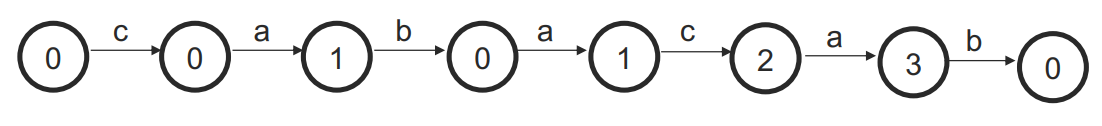
\includegraphics[width=0.5\textwidth]{img/pattern/ScansioneTesto.png}
        \caption{Risultato della scansione del testo}
        \label{fig:scansione}
    \end{figure}
\end{esempio}
A questo punto è necessario identificare un'occorrenza esatta del pattern $P$ nel
testo $T$. Per risolvere questo, partiamo dalla successione di stati che abbiamo
definito per la scansione del testo. Essa corrisponde a una successione di posizioni
su $P$, o in altre parole, a una successione di lunghezze di prefissi del pattern $P$.
\begin{teorema}
    $j_i$, con $0 \leq i \leq n$, è la lunghezza del \textbf{più lungo} prefisso
    di $P$ uguale a una sottostringa di $T$ che finisce in posizione $i$.
\end{teorema}
\begin{dimostrazione}
    È possibile dimostrare il teorema precedente con una dimostrazione per induzione:
    \begin{enumerate}
        \item \textbf{Caso base}: per lo stato $j_0 = 0$ il teorema è banalmente
              dimostrabile, in quanto il prefisso di lunghezza $0$ è il prefisso nullo
              che è sottostringa di $T$.
        \item \textbf{Passo induttivo}: se $j_{i-1}$ è la lunghezza del più lungo
              prefisso di $P$ uguale alla sottostringa di $T$ che finisce in posizione
              $i-1$, allora $j_i$ è la lunghezza del più lungo prefisso di $P$ uguale
              alla sottostringa di $T$ che finisce in posizione $i$.

              Per dimostrare il passo induttivo ci basiamo sulla seguente ipotesi:
              $j_{i-1}$ è la lunghezza del più lungo prefisso di $P$ uguale a una
              sottostringa di $T$ che finisce in posizione $i-1$.
              \begin{itemize}
                  \item \textbf{Caso 1}: $j_{i - 1} < m$ e $P[j_{i - 1} + 1] = T[i]$
                        questo implica $j_i = \delta(j_{i - 1}, T[i]) = j_{i - 1} + 1$
                        \begin{itemize}
                            \item $j_{i - 1} \neq 0$: la tesi è confermata
                            \item $j_{i - 1} = 0$ vuol dire che il carattere
                                  corrisponde con il carattere iniziale del pattern
                        \end{itemize}
                  \item \textbf{Caso 2}: $j_{i - 1} = m$ oppure
                        $P[j_{i - 1} + 1] \neq T[i]$ questo implica
                        $j_i = \delta(j_{i - 1}, T[i]) = k$ dove $k$ è la lunghezza del
                        bordo di $P[1, j_{i - 1}]T[i]$.
                        \begin{itemize}
                            \item $0 < j_{i - 1} < m$: in questo caso il valore
                                  di $k$ mi rappresenta una parte del testo per cui ho
                                  già verificato un'occorrenza esatta, questo mi viene
                                  garantito dalla definizione di bordo.
                            \item $j_{i - 1} = 0$ vuol dire che sono rimasto nello stato 0.
                            \item $j_{i - 1} = m$ ho trovato un'occorrenza esatta
                                  del pattern, inoltre per evitare di perdere delle
                                  occorrenze mi sposto in base alla lunghezza del bordo
                                  del pattern concatenato con il carattere successivo.
                        \end{itemize}
              \end{itemize}
    \end{enumerate}
\end{dimostrazione}
Questo teorema mi fornisce la garanzia che non sto perdendo delle occorrenze.
Inoltre, posso trovare la posizione di inizio dell'occorrenza esatta come $i - j + 1$.
Nel caso in cui $j_i = m$ ho identificato un'occorrenza esatta del pattern $P$.

Possiamo riassumere la scansione del testo come:
\begin{enumerate}
    \item Si parte dallo stato iniziale $0$ e si effettua una scansione di $T$
          dal primo all'ultimo simbolo.
    \item Per ogni posizione $i$ di $T$ si effettua la transizione dallo stato
          corrente $j_c$ al nuovo stato $j_f = \delta(j_c, T[i])$
    \item Ogni volta che lo stato $j_f$ è lo stato accettante ($m$), viene prodotta
          in output l'occorrenza $i - m + 1$
\end{enumerate}
\begin{algorithm}
    \begin{algorithmic}
        \Function{ASF\_exact\_occurrences}{$\delta, T, m$}
        \State $n \gets |T|$
        \State $j \gets 0$
        \For{$i \gets 1 \ \text{to} \ n$}
        \State $j \gets \delta(j, T[i])$
        \If{$j = m$}
        \State $\text{\textbf{Output}} \ i - m + 1$
        \EndIf
        \EndFor
        \EndFunction
    \end{algorithmic}
    \caption{Algoritmo per la ricerca esatta con Automa a Stati Finiti}
\end{algorithm}
Questo algoritmo viene eseguito in tempo $\theta(n)$.
\begin{esempio}
    Consideriamo il testo $T$:
    \begin{table}[!ht]
        \centering
        \begin{tabular}{ccccccccccccc}
            1                       & 2                      & 3                      & 4                      & 5                      & 6                      & 7                      & 8                      & 9                      & 10                     & 11                     & 12                     & 13                     \\ \hline
            \multicolumn{1}{|c|}{c} & \multicolumn{1}{c|}{a} & \multicolumn{1}{c|}{b} & \multicolumn{1}{c|}{a} & \multicolumn{1}{c|}{c} & \multicolumn{1}{c|}{a} & \multicolumn{1}{c|}{c} & \multicolumn{1}{c|}{b} & \multicolumn{1}{c|}{a} & \multicolumn{1}{c|}{c} & \multicolumn{1}{c|}{a} & \multicolumn{1}{c|}{b} & \multicolumn{1}{c|}{a} \\ \hline
        \end{tabular}
    \end{table}

    e il pattern $P$:
    \begin{table}[!ht]
        \centering
        \begin{tabular}{ccccccc}
            1                       & 2                      & 3                      & 4                      & 5                      & 6                      & 7                      \\ \hline
            \multicolumn{1}{|c|}{a} & \multicolumn{1}{c|}{c} & \multicolumn{1}{c|}{a} & \multicolumn{1}{c|}{c} & \multicolumn{1}{c|}{b} & \multicolumn{1}{c|}{a} & \multicolumn{1}{c|}{c} \\ \hline
        \end{tabular}
    \end{table}

    Su cui è stata definita la seguente funzione di transizione $\delta$:
    \begin{table}[!ht]
        \centering
        \begin{tabular}{|>{\columncolor[HTML]{EFEFEF}}c |c|c|c|}\hline
            $\delta$   & \cellcolor[HTML]{EFEFEF}\textbf{a} & \cellcolor[HTML]{EFEFEF}\textbf{b} & \cellcolor[HTML]{EFEFEF}\textbf{c} \\ \hline
            \textbf{0} & 1                                  & 0                                  & 0                                  \\ \hline
            \textbf{1} & 1                                  & 0                                  & 2                                  \\ \hline
            \textbf{2} & 3                                  & 0                                  & 0                                  \\ \hline
            \textbf{3} & 1                                  & 0                                  & 4                                  \\ \hline
            \textbf{4} & 3                                  & 5                                  & 0                                  \\ \hline
            \textbf{5} & 6                                  & 0                                  & 0                                  \\ \hline
            \textbf{6} & 1                                  & 0                                  & 7                                  \\ \hline
            \textbf{7} & 3                                  & 0                                  & 0                                  \\ \hline
        \end{tabular}
    \end{table}

    Otteniamo la seguente esecuzione dell'algoritmo:
    \begin{figure}[!ht]
        \centering
        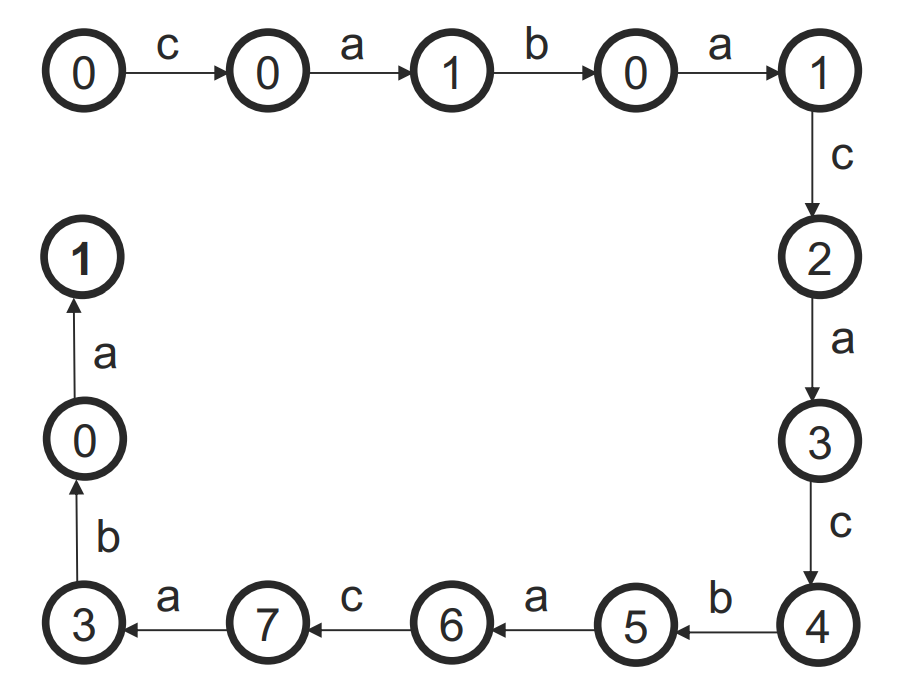
\includegraphics[width=0.3\textwidth]{img/pattern/ASF.png}
        \caption{Esecuzione dell'algoritmo per la ricerca esatta con Automa a Stati Finiti}
        \label{fig:enter-label}
    \end{figure}
\end{esempio}
\subsection{Calcolo della funzione di transizione $\delta$}
L'algoritmo più semplice che permette di calcolare i valori della funzione di
transizione $\delta$ consiste nell’applicare la funzione di transizione $\delta$ per
come è definita senza sfruttare i valori che sono già stati computati.
\begin{algorithm}
    \begin{algorithmic}
        \Function{Trivial-build-transition-function}{$P$}
        \State $m\gets |P|$
        \State $\delta \gets empty\_table (m + 1) \times | \Sigma|$
        \For{$j \gets 0 \ \text{to} \ m - 1$}
        \State $\delta(j, P[j + 1]) \gets j + 1$
        \EndFor
        \For{$j \gets 0 \ \text{to} \ m$}
        \For{$\sigma \in \Sigma$}
        \State $\delta(j, \sigma) \gets |B(P[1, j]\sigma)|$
        \EndFor
        \EndFor
        \State $\text{\textbf{return}} \ \delta$
        \EndFunction
    \end{algorithmic}
    \caption{Algoritmo banale per il calcolo della funzione di transizione $\delta$}
\end{algorithm}
Questo algoritmo richiede un tempo nel caso peggiore pari a $\mathcal{O}(m^3 | \Sigma|)$,
questo è dovuto al fatto che per calcolare il bordo è necessario un tempo, nel
caso peggiore pari a $\mathcal{O}(m^2)$.

Definiamo $\delta_j$ come la funzione di transizione di $P[1, j]$, ovvero come
una funzione:
\begin{equation}
    \delta_j: \{0, 1, \dots, j\} \times \Sigma \to \{0, 1, \dots, j\}
\end{equation}
per questa funzione possiamo definire due casi particolari:
\begin{itemize}
    \item $\delta_0$ ovvero la funzione di transizione di $P[1, 0]$ che per
          definizione è $\varepsilon$, quindi il valore di tale funzione è sempre $0$.
    \item $\delta_m$ ovvero la funzione di transizione di $P[1, m]$ la quale
          corrisponde precisamente alla funzione di transizione del pattern $P$.
\end{itemize}
Possiamo definire il calcolo della funzione di transizione $delta$ per un pattern
$P$ di lunghezza $m$ utilizzando l'induzione nel seguente modo:
\begin{itemize}
    \item Caso base: calcolo $\delta_0$
    \item Passo induttivo: calcolo $\delta_j$ da $\delta_{j - 1}$ in questo caso
          dobbiamo distinguere il caso in cui $j = 1$ e i restanti.
          \begin{itemize}
              \item Nel caso in cui $j = 1$, possiamo definire la funzione di
                    transizione come:
                    \begin{enumerate}
                        \item Prendo il valore $0$ contenuto nella cella della
                              riga $0$ di $\delta_0$ in corrispondenza del simbolo $P[1]$
                        \item Sostituisco il valore $0$ con il valore $1$ (stato
                              successivo a $0$).
                        \item Aggiungo una nuova riga (corrispondente allo stato $1$)
                        \item Copio la riga che corrisponde allo stato 0 nella riga
                              che corrisponde allo stato $1$
                        \item Rinomino $\delta_0$ in $\delta_1$
                    \end{enumerate}
              \item Mentre nel caso in cui $j \neq 1$ possiamo definire la
                    funzione di transizione come:
                    \begin{enumerate}
                        \item Prendo il valore $k$ contenuto nella cella della
                              riga $j-1$ di $\delta_{j-1}$ in corrispondenza del simbolo $P[j]$
                        \item Sostituisco il valore $k$ con il valore $j$ (stato
                              successivo a $j - 1$)
                        \item Aggiungo una nuova riga (corrispondente allo stato $j$)
                        \item Copio la riga che corrisponde allo stato $k$ nella
                              riga che corrisponde allo stato $j$
                        \item Rinomino $\delta_{j-1}$ in $\delta_j$
                    \end{enumerate}
          \end{itemize}
\end{itemize}
\begin{nota}
    Dimostrazione tramite esempi su slide.
\end{nota}
Con queste informazioni possiamo definire un algoritmo che mi permette di calcolare
la funzione di transizione $\delta$ in tempo $\theta(m \cdot |\Sigma|)$. Tale
algoritmo sfrutta le informazioni precedentemente calcolate.
\begin{algorithm}[!ht]
    \begin{algorithmic}
        \Function{Build-transition-function}{$P$}
        \State $m\gets |P|$
        \State $\delta \gets empty\_table (m + 1) \times | \Sigma|$
        \For{$\sigma \in \Sigma$}
        \State $\delta(0, \sigma) \gets 0$
        \EndFor
        \For{$j \gets 1 \ \text{to} \ m$}
        \State $k \gets \delta(j - 1, P[j])$
        \State $\delta(j - 1, P[j]) \gets j$
        \For{$\sigma \in \Sigma$}
        \State $\delta(j, \sigma) \gets \delta(k, \sigma)$
        \EndFor
        \EndFor
        \State $\text{\textbf{return}} \ \delta$
        \EndFunction
    \end{algorithmic}
    \caption{Algoritmo per il calcolo della funzione di transizione $\delta$}
\end{algorithm}
\newpage
\section{Algoritmo di Knuth-Morris-Pratt}
Questo algoritmo per la ricerca esatta è basato su un'analisi del pattern. Si hanno due fasi:
\begin{enumerate}
    \item \textbf{Preprocessing del pattern}: questa fase consiste nel calcolo
          della prefix function $\phi$, che è una funzione che associa ad ogni posizione
          del pattern la lunghezza del più lungo prefisso del pattern che è anche un
          suffisso del pattern. Questa funzione è calcolata in tempo lineare rispetto
          alla lunghezza del pattern $\mathcal{O}(m)$.
    \item \textbf{Scansione del testo}: questa fase consiste nel confrontare il
          pattern con il testo cercando di identificare le occorrenze esatte di esso.
          Questa fase è eseguita in tempo lineare rispetto alla lunghezza del testo $\mathcal{O}(n)$.
\end{enumerate}
La \textbf{prefix function} o funzione di fallimento $\phi$ è definita come segue:
\begin{equation}
    \phi: \{0, 1, \dots m\} \to \{-1, 0, \dots m\}
\end{equation}
Essa è definita come segue:
\begin{equation}
    \phi(j) = \begin{cases} |B(P[1, j])| & \text{se } 1 \leq j \leq m \\-1 & \text{se } j = 0 \end{cases}
\end{equation}

\begin{esempio}
	Calcoliamo $\phi$ sul pattern $P=abcabaabcabab$ con $m=13$.
    \begin{table}[!ht] 
        \centering
        \begin{tabular}{|>{\columncolor[HTML]{EFEFEF}}c|c|c|c|c|c|c|c|c|c|c|c|c|c|c|}\hline
            \cellcolor[HTML]{EFEFEF}\textbf{j}&\cellcolor[HTML]{EFEFEF}\textbf{0}
            &\cellcolor[HTML]{EFEFEF}\textbf{1}&\cellcolor[HTML]{EFEFEF}\textbf{2}
            &\cellcolor[HTML]{EFEFEF}\textbf{3}&\cellcolor[HTML]{EFEFEF}\textbf{4}
            &\cellcolor[HTML]{EFEFEF}\textbf{5}&\cellcolor[HTML]{EFEFEF}\textbf{6}
            &\cellcolor[HTML]{EFEFEF}\textbf{7}&\cellcolor[HTML]{EFEFEF}\textbf{8}
            &\cellcolor[HTML]{EFEFEF}\textbf{9}&\cellcolor[HTML]{EFEFEF}\textbf{10}
            &\cellcolor[HTML]{EFEFEF}\textbf{11}&\cellcolor[HTML]{EFEFEF}\textbf{12}
            &\cellcolor[HTML]{EFEFEF}\textbf{13}\\	\hline
            $\phi$& -1&0&0&0&1&2&1&1&2&3&4&5&6&2\\\hline
        \end{tabular}
    \end{table}	

\end{esempio}

Questo algoritmo è un’evoluzione dell'algoritmo banale per la ricerca delle 
occorrenze di un pattern in un testo. In particolare, l'algoritmo KMP consiste in:
\begin{enumerate}
    \item Viene usata una finestra $W$ di lunghezza $m$ che scorre sul testo $T$
          da sinistra a destra con posizione iniziale $i = 1$.
    \item Si confrontano i simboli di $P$ con i corrispondenti simboli di $T$
          all'interno della finestra $W$ andando da sinistra a destra e partendo
          dal primo simbolo di $P$.
    \item Non appena si incontra un mismatch oppure ogni simbolo di $P$ ha un
          match con il corrispondente simbolo in $W$ (i è occorrenza esatta), $W$ viene
          spostata a destra nella posizione $p = i + j - \phi(j - 1) - 1$, dove $j$ è
          l'indice del simbolo di $P$ che ha causato il mismatch, mentre $i$ è
          la posizione iniziale di $W$.
    \item L'ultima posizione di $W$ è $n - m + 1$.
\end{enumerate}
Riassumendo:
\begin{itemize}
    \item $W$ viene spostata dalla posizione $i$ alla posizione $p$, dove:
          $$p = i + j - \phi(j - 1) - 1$$ con $j$ indice del simbolo di $P$ che ha
          causato il mismatch per $W$ in posizione $i$.
    \item Il confronto riparte dal simbolo di $P$ in posizione $j = \phi(j - 1) + 1$
          e dal simbolo di $T$ in posizione $i + j - 1$.
\end{itemize}
Nel caso in cui $j = 1$, allora $p = i + 1$ e il confronto riparte dal primo
simbolo di $P$ e dal simbolo di $T$ in posizione $i + 1$.
\begin{nota}
    Chiaramente il confronto riparte dalle posizioni $i + 1$ su $T$ e $1$ su P,
    ma dire che riparte dalla posizione $i$ su $T$ e dalla posizione $0$ su $P$
    implicitamente fa riferimento ad un confronto iniziale fittizio tra $T[i]$ e
    $P[0]$ (simbolo inesistente) che di default viene considerato un match.
\end{nota}
Nel caso in cui $j = m + 1$, allora $p = i + m - \phi(m) - 1$ e il confronto
riparte dal primo simbolo di $P$ e dal simbolo di $T$ in posizione $i + m - \phi(m)$.

\begin{table}[!ht]
    \centering
    \begin{tabular}{|l|l|l|}
        \hline
                           & Automa a stati finiti       & KMP              \\ \hline
        Preprocessing di P & $\mathcal{O}(m | \Sigma |)$ & $\mathcal{O}(m)$ \\ \hline
        Scansione di T     & $\mathcal{O}(n)$            & $\mathcal{O}(n)$ \\ \hline
        Spazio             & $\mathcal{O}(m | \Sigma |)$ & $\mathcal{O}(m)$ \\ \hline
    \end{tabular}
\end{table}
Le differenze tra l'algoritmo basato sull'automa e KMP sono:
\begin{itemize}
    \item Automa:
    \begin{itemize}
        \item Efficiente per pattern piccoli, perché la memoria è contenuta 
        quindi le costanti all'interno del calcolo del tempo sono migliori.
        \item Richiede più tempo e memoria per pattern grandi, perché sprechiamo
         tempo nel calcolo del $\delta$.
        \item Ricerca di P in testi diversi utilizzando lo stesso automa
    \end{itemize}
    KMP:
    \begin{itemize}
        \item Efficiente per pattern grandi
        \item Richiede più tempo per pattern piccoli
    \end{itemize}
\end{itemize}

%% Mettere il codice solo se lo chiede
\section{Algoritmo di Baeza-Yates e Gonnet}
La ricerca esatta effettuata attraverso questo algoritmo effettua un confronto
tra i simboli del pattern e del testo in maniera non esplicita, ovvero non confronta
carattere per carattere. In questo algoritmo vengono effettuate in parallelo operazioni
bit a bit su word di bit, viene anche chiamato \textit{algoritmo bit parallel}.

Questo algoritmo segue il paradigma \textbf{shift-and} ovvero compie fondamentalmente
due sole operazioni:
\begin{itemize}
    \item \textbf{Shift} dei bit.
    \item \textbf{AND} logico tra i bit.
\end{itemize}
Come gli algoritmi visti fin ora, anche in questo caso possiamo descrivere il suo
funzionamento attraverso due fasi:
\begin{itemize}
    \item \textbf{Preprocessing del pattern} $P$ nel quale vengono calcolate 
    $|\Sigma|$ \textbf{words} ognuna di $m$ bit. Questa operazione viene eseguita 
    in tempo $\theta(|\Sigma| + m)$.
    \item \textbf{Scansione del testo} $T$ per cercare le occorrenze esatte del 
    pattern $P$. Questa operazione viene eseguita in tempo $\theta(n)$.
\end{itemize}
\subsection{Word e Operatori}
\begin{definizione}[\textbf{Word di bit}]
    Una \textbf{word di bit} è un gruppo di bit che viene trattato come un'unità
    la cui dimensione può variare e che rappresenta un valore di un certo tipo,
    come ad esempio un numero o un carattere. In una word, il bit più a destra è
    quello meno significativo, mentre quello più a sinistra è quello più significativo.
\end{definizione}
Sulle word si possono eseguire delle operazioni \textit{bit a bit}, ovvero si
esegue un'operazione tra i bit corrispondenti di due o più words di bit della
stessa lunghezza. Il valore restituito da queste operazioni è una nuova word in
cui ogni bit è il risultato dell'operazione tra i bit corrispondenti nelle word
in input. Tra queste operazioni abbiamo:
\begin{itemize}
    \item \textbf{Congiunzione logica} $\to$ AND. Questa operazione è implementata come:
          \begin{equation}
              w = w_1 \ \text{AND} \ w_2
          \end{equation}
          restituisce una word $w$ tale che:
          \begin{itemize}
              \item $w[j] = 1$ se e solo se $w_1[j] \ \text{AND} \ w_2[j] =  1$.
              \item $w[j] = 0$ altrimenti.
          \end{itemize}
    \item \textbf{Disgiunzione logica} (inclusiva) $\to$ OR. Questa operazione è 
    implementata come:
          \begin{equation}
              w = w_1 \ \text{OR} \ w_2
          \end{equation}
          restituisce una word $w$ tale che:
          \begin{itemize}
              \item $w[j] = 1$ se e solo se $w_1[j] \ \text{OR} \ w_2[j] =  1$.
              \item $w[j] = 0$ altrimenti.
          \end{itemize}
    \item \textbf{Shift dei bit} di una posizione a destra con bit più significativo a $0$
          $\to$ RSHIFT. Questa operazione è implementata come:
          \begin{equation}
              w = \text{RSHIFT}(w_1)
          \end{equation}
          restituisce una word $w$ tale che:
          \begin{itemize}
              \item $w[j] = w_1[j - 1]$ se $j \geq 2$.
              \item $w[1] = 0$ altrimenti.
          \end{itemize}
    \item \textbf{Shift dei bit} di una posizione a destra con bit più significativo a $1$
          $\to$ RSHIFT1. Questa operazione viene implementata come un RSHIFT seguito
          da un OR con una maschera in cui nella prima posizione è presente 1 e nelle altre 0.
\end{itemize}
\subsection{Preprocessing del pattern}
Dato un pattern di lunghezza $m$ e $\sigma$ in $\Sigma$, $B_{\sigma}$ è una word di $m$ bit tale che:
\begin{equation}
    B_{\sigma}[j] = 1 \iff P[j] = \sigma
\end{equation}
Viene creata una word per ogni simbolo dell'alfabeto $\Sigma$ e viene memorizzata
in una tabella $B$. Con questa rappresentazione posso effettuare le query del tipo:
"il simbolo in posizione $j$ di $P$ è uguale a un certo simbolo $\sigma$".
\begin{esempio}
	Calcoliamo la tabella $B$ per un pattern $P=abcaba$ su un alfabeto $\Sigma=\left\{a,b,c,d\right\}$.
    \begin{table}[!ht]
        \centering
        \begin{tabular}{|c|c|c|c|c|c|c|}
        \hline
            P & $a$ & $b$ & $c$ & $a$ & $b$ & $a$\\ \hline
            $B_a$ & $1$ & $0$ & $0$ & $1$ & $0$ & $1$ \\ \hline
            $B_b$ & $0$ & $1$ & $0$ & $0$ & $1$ & $0$ \\ \hline
            $B_c$ & $0$ & $0$ & $1$ & $0$ & $0$ & $0$ \\ \hline
            $B_d$ & $0$ & $0$ & $0$ & $0$ & $0$ & $0$ \\ \hline
        \end{tabular}
    \end{table}
\end{esempio}
Vediamo ora come calcolare la tabella $B$:
\begin{enumerate}
    \item tutte le word $B_{\sigma}$ vengono inizializzate a $m$ bit a $0$.
    \item viene creata una maschera $M$ di $m$ bit tutti uguali a $0$ tranne il
          più significativo che è uguale a $1$.
    \item si esegue una scansione di $P$ da sinistra a destra, e per ogni posizione
          $j$ vengono eseguite le due operazioni bit a bit:
          \begin{itemize}
              \item $B_{P[j]} = M \ \textbf{OR} \ B_{P[j]}$
              \item $M = \textbf{RSHIFT} (M)$
          \end{itemize}
\end{enumerate}
L'algoritmo per calcolare la tabella richiede un tempo pari a $\theta(|\Sigma| + m)$ ed è il seguente:
\begin{algorithm}
    \begin{algorithmic}
        \Function{Compute-table-B}{$P$}
        \State $m \gets |P|$
        \State $B \gets \text{empty table of} \ |\Sigma| \ \text{words} \ B_{\sigma}$
        \For{$\sigma \in \Sigma$}
        \State $B_{\sigma} \gets 00\dots0$
        \EndFor
        \State $M \gets 10\dots0$
        \For{$\sigma \in \Sigma$}
            \State $\sigma \gets P[j]$
            \State $B_{\sigma} \gets M \ \text{OR} \ B_{\sigma}$
            \State $M = \textbf{RSHIFT} (M)$
        \EndFor
        \State \textbf{return} $B$
        \EndFunction
    \end{algorithmic}
    \caption{Algoritmo per il calcolo della tabella $B$}
\end{algorithm}
\subsection{Scansione del testo}
La procedura per la scansione del testo è rappresentata come:
\begin{enumerate}
    \item Il testo $T$ viene scandito dalla prima all'ultima posizione.
    \item Per ogni posizione $i$ del testo $T$ viene calcolata una word $D_i$ di $m$ bit.
    \item Ogni volta che in $D_i$ il bit meno significativo è uguale a $1$, allora
          $i - m + 1$ è occorrenza esatta di $P$ in $T$.
\end{enumerate}
Dobbiamo ora definire cosa si intende con la word $D_i$. Prima di fare ciò dobbiamo
definire $P[1,j] = suff(T[1,i])$ ovvero $P[1,j]$ è uguale a un suffisso di $T[1,i]$.
\begin{definizione}[\textbf{Word $D_i$}]
    Dati $P$ lungo $m$ e $T$ lungo $n$, $D_i$ ($0 \leq i \leq n$) è una word di
    $m$ bit tale che:
    \begin{equation}
        D_i[j] = 1 \iff P[1,j] = suff(T[1,i])
    \end{equation}
    Inoltre, sappiamo per definizione che:
    \begin{itemize}
        \item $D_0 = 00\dots0$ dato che $P[1, j] \neq suff(T[1, 0]) \ \forall j$
        \item $D_i[m] = 1$ se e solo se $P[1, m] = suff(T[i-m + 1, i])$ ovvero
              si ha un’occorrenza esatta di $P$ in $T$ nella posizione $i - m + 1$.
    \end{itemize}
\end{definizione}
Ovviamente calcolare $D_i$ è sempre troppo costoso, infatti, $D_i$ viene sempre 
ottenuto a partire da $D_{i-1}$, portando a modificare l'algoritmo di scansione 
del testo nel seguente modo:
\begin{itemize}
    \item Inizia dalla word $D_0 = 00\dots0$
    \item Per ogni $i$ da $1$ a $n$ calcola la word $D_i$ a partire dalla word $D_{i-1}$.
    \item Ogni volta che $D_i$ ha il bit meno significativo uguale a $1$, viene
          prodotta in output l'occorrenza $i- m + 1$.
\end{itemize}
Vediamo ora come si calcola il valore di $D_i$ a partire da $D_{i - 1}$:
\begin{itemize}
    \item Se $j =  1$ allora posso calcolarla come:
    \begin{equation}
        D_i[1] = 1 \text{\textbf{AND}} B_{T[i]}[1]
    \end{equation}
    Perché $D_i[1] = 1\iff P[1,1] =suff(T[1,i])\iff P[1] = T[i]\iff B_{T[i]}[1]$.
    Si aggiunge $1$ per semplificare le operazioni bit a bit. 
    \item Se $J =  1$ allora posso calcolarla come:
          \begin{equation}
              D_i[j] = 1 \text{\textbf{AND}} B_{T[i]}[1]
          \end{equation}
          Si aggiunge $1$ per semplificare le operazioni bit a bit.
    \item Se $j > 1$ allora posso calcolarla come:
    \begin{equation}
        D_i[j] = D_{i - 1}[j - 1] \text{\textbf{AND}} B_{T[i]}[j]
    \end{equation}
    Perché $D_i[j] = 1 \iff P[1,j] = suff(T[1,i]) \iff P[1,j-1] = suff(T[1,i-1])
     \text{\textbf{AND}} P[j] = T[i] \iff D_{i-1}[j-1] \text{\textbf{AND}} B_{T[i]}[j]$.
\end{itemize}
In questo modo stiamo ancora aggiornando un bit alla volta, ma sfruttando le 
operazioni bit a bit si possono aggiornare tutti in tempo \textbf{costante} nel seguente modo:
\begin{equation}
    D_i = \text{\textbf{RSHIFT1}}(D_{i - 1}) \ \text{\textbf{AND}} \ B_{T[i]}
\end{equation}
Vediamo ora come implementare l'algoritmo che effettua la scansione del testo in tempo $\theta(n)$
\begin{algorithm}
    \begin{algorithmic}
        \Function{BYG}{$B, T$}
        \State $n \gets |T|$
        \State $D \gets 00\dots0$
        \State $M \gets 00\dots01$
        \For{$i \gets 1 \ \text{to} \ n$}
        \State $\sigma \gets T[i]$
        \State $D \gets \text{\textbf{RSHIFT1}}(D_{i - 1}) \ \text{\textbf{AND}} \ B_{T[i]}$
        \If{$(D \ \text{\textbf{AND}} M) = M$}
        \State \text{output} $i - m + 1$
        \EndIf
        \EndFor
        \EndFunction
    \end{algorithmic}
    \caption{Algoritmo per la scansione del testo}
\end{algorithm}

\begin{esempio}
	Siano un testo $T=babcabaadc$ e un pattern $P=abcaba$ tale che $|T| = 10$ e $|P|=6$.
     Entrambe le stringhe costruite sun un alfabeto $\Sigma=\left\{a,b,c,d\right\}$, 
	allora costruiamo la tabella $B_\sigma$: 
    \begin{table}[!ht]
        \centering
        \begin{tabular}{|c|c|c|c|c|c|c|}
        \hline
            P & $a$ & $b$ & $c$ & $a$ & $b$ & $a$\\ \hline
            $B_a$ & $1$ & $0$ & $0$ & $1$ & $0$ & $1$ \\ \hline
            $B_b$ & $0$ & $1$ & $0$ & $0$ & $1$ & $0$ \\ \hline
            $B_c$ & $0$ & $0$ & $1$ & $0$ & $0$ & $0$ \\ \hline
            $B_d$ & $0$ & $0$ & $0$ & $0$ & $0$ & $0$ \\ \hline
        \end{tabular}
    \end{table}
    I singoli passi sono i seguenti:
    \begin{itemize}
        \item Quindi partiremo da $D_0 = 000000$, leggo il primo simbolo del testo $T[1] = b$ e poi calcolo
        $$D_1=RSHIFT1(D_{0}) \text{ AND } B_b = 100000 \text{ AND } 010010 = 000000$$
        \item leggo il secondo simbolo del testo $T[2] = a$ e poi calcolo $D_2$
        $$D_2 = 100000 \text{ AND } 100101 = 100000 $$
        \item leggo il secondo simbolo del testo $T[3] = b$ e poi calcolo $D_3$
        $$D_3 = 110000 \text{ AND } 010010 = 010000 $$
        \item leggo il secondo simbolo del testo $T[4] = c$ e poi calcolo $D_4$
        $$D_4 = 101100 \text{ AND } 001000 = 001000 $$
        \item leggo il secondo simbolo del testo $T[5] = a$ e poi calcolo $D_5$
        $$D_5 = 100100 \text{ AND } 100101 = 100100 $$
        \item $\dots$
        \item leggo il secondo simbolo del testo $T[7] = a$ e poi calcolo $D_7$
        $$D_6 = 101001 \text{ AND } 100101 = 100001 $$
        \item Ho il bit LSB di $D_6$ uguale a $1$, quindi ho trovato un match che
         corrisponde a $i-m+1 =7-6+1= 2$. Poi continuo fino a quando non termino $T$.
    \end{itemize}
\end{esempio}


\section{Algoritmo di Wu e Manber}
L'algoritmo risolvere problemi di \textbf{stringmatching approssimati} e il funzionamento
è simile a \textbf{BYG}.
Riprendiamo la definizione di ricerca approssimata di un pattern $P$ in un testo $T$:
\begin{definizione}[\textbf{Occorrenza approssimata}]
    Una posizione $i$ del testo $T$ tale che esista una sottostringa $S =T[i - L + 1]$
    tale che $ED(P, S) \leq k$ è detta \textbf{occurrenza approssimata} di $P$ in $T$.
\end{definizione}

Come gli algoritmi visti fino a questo momento, quello di Wu e Manber è basato su due fasi:
\begin{enumerate}
    \item \textbf{prepocessing} del pattern $P$ nel quale vengono calcolate $|\Sigma|$
          \textbf{words} ognuna di $m$ bit. Questa operazione viene eseguita in tempo
          $\theta(|\Sigma| + m)$. (\textit{uguale a quello dell'algoritmo BYG})
    \item \textbf{Scansione del testo} $T$ per cercare le occorrenze approssimate del pattern $P$.
          Questa operazione viene eseguita in tempo $\theta(k \cdot n)$.
\end{enumerate}
\subsection{Scansione del testo}
Dato che la fase di preprocessing è equivalente a quella per l'algoritmo BYG,
passiamo subito alla scansione del testo. Per fare ciò dobbiamo definire la word
$D_i^h$, con $0 \leq h \leq k$ e $0 \leq i \leq n$.

Partiamo definiendo $P[1, j] = suff_h(T[1, i])$ ovvero $P[1, j]$ è uguale a un
suffisso di $T[1, i]$ a meno di $h$ errori. In altre parole, riesco a trovare un
suffisso $S$ di $T[1, i]$ tale che $ED(P[1, j], S) \leq h$.

Estenderemo la definizione di $D_i$ di ShiftAND al caso in cui si ammettono al più $h$ errori.
\begin{definizione}[\textbf{Word $D_i^h$}]
    Dati un pattern $P$ lungo $m$, un testo $T$ lungo $n$ e una soglia di errore $k$,
    possiamo definire la \textbf{word $D_i^h$} come una word di $m$ bit tale che:
    \begin{equation}
        D_i^h[j] = 1 \iff P[1, j] = suff_h(T[1, i])
    \end{equation}
\end{definizione}
Vediamo ora alcuni casi particolare:
\begin{itemize}
    \item $D_i^0$: ovvero la la word con $h = 0$, è per definizione la word $D_i$
          dell'algoritmo BYG.
    \item $D_0^h$: ovvero la word con $i = 0$, è tale che:
          \begin{itemize}
              \item $j \leq h \implies D_0^h[j] = 1$, questo perché $P[1, j]$ è un
                    prefisso di $T[1, 0]$ e quindi $ED(P[1, j], T[1, 0]) \leq h$.
              \item $j > h \implies D_0^h[j] = 0$, questo perché $P[1, j]$ non è un
                    prefisso di $T[1, 0]$ e quindi $ED(P[1, j], T[1, 0]) > h$.
          \end{itemize}
          Si ottiene quindi una word dove i primi $h$ bit sono uguali a $1$ e i
          restanti $m - h$ bit sono posti a $0$.
    \item $D_i^h [m] = i \iff P[1, m] = suff_h(T[1, i])$, ovvero se $P[1, m]$ è un
          suffisso di $T[1, i]$ a meno di $h$ errori, allora $D_i^h[m] = 1$. Nel
          caso particolare in cui $h = 0$ si ha un occorrenza esatta in $i - m + 1$.
          Mentre nel caso in cui $h = k$ si ha un'occorrenza approssimata in posizione $i$.
\end{itemize}
\begin{nota}
    In generale, $D_i^{h'}[j] = 1$ implica $D_i^{h}[j] = 1$ con $h > h'$. Inoltre,
    $D_{i}^{h} [j] = 1$ implica $D_{i}^{h + 1}[j + 1] = 1$ e $D_{i}^{h + 1}[j - 1] = 1$
\end{nota}
Definita la word $D_i^h$, possiamo definire la scansione del testo $T$ come una
successione di $k + 1$ scansioni, dove solamente all'iterazione $k$ si vanno a
verificare i bit finali delle word per cercare l'occorrenza approssimata.
Nello specifico, se all'iterazione $k$ si ha che $D_i^k[m] = 1$, allora si ha in
output l'occorrenza approssimata $i$.

Fino ad ora abbiamo definito come calcolare il caso in cui $h = 0$ oppure il caso
in cui $i = 0$. Vediamo ora come calcolare il caso in cui $i > 0, h > 0$.

Partiamo considerando il caso in cui $j > 1$, in questa situazione abbiamo che:
\begin{equation}
    D_i^h[j] = 1 \iff P[1, j] =suff_h(T[1, i]) \Leftarrow P[1, j - 1] = suff_h(T[1, i - 1]) \  \textbf{AND} \ T[i] = P[j]
\end{equation}
ovvero $D_i^h[j] = 1$ se e solo se $P[1, j - 1]$ è un suffisso di $T[1, i - 1]$
a meno di $h$ errori e $T[i] = P[j]$. Questo significa che $D_i^h[j] = 1$ se e solo se:
\begin{equation}
    D_{i - 1}^h[j - 1] = D_{i - 1}^h [j - 1] = 1 \ \textbf{AND} \ B_{T[i]} [j] =  1
\end{equation}
Quello appena visto non è l'unico caso, infatti possiamo avere anche:
\begin{equation}
    D_i^h[j] = 1 \iff P[1, j] =suff_h(T[1, i]) \Leftarrow P[1, j - 1] = suff_{h - 1}(T[1, i - 1])
\end{equation}
ovvero non ho ancora raggiunto il limite di errori e quindi posso ancora avere
errori senza superare la soglia $h$. Questo significa che $D_i^h[j] = 1$ se e solo se:
\begin{equation}
    D_i^h[j] = 1 \Leftarrow D_{i - 1}^{h - 1} [j - 1] = 1
\end{equation}
Un altra casistica è data dal fatto che posso avere un carattere in meno nel testo,
ottenendo quindi:
\begin{equation}
    D_i^h[j] = 1 \iff P[1, j] =suff_h(T[1, i]) \Leftarrow P[1, j] = suff_{h - 1}(T[1, i - 1])
\end{equation}
ovvero non ho ancora raggiunto il limite di errori. Questo significa che $D_i^h[j] = 1$
se e solo se:
\begin{equation}
    D_i^h[j] = 1 \Leftarrow D_{i - 1}^{h - 1} [j] = 1
\end{equation}
Il quarto e ultimo caso è dato dal fatto che posso modificare il pattern, ovvero:
\begin{equation}
    D_i^h[j] = 1 \iff P[1, j] =suff_h(T[1, i]) \Leftarrow P[1, j - 1] = suff_{h - 1}(T[1, i])
\end{equation}
ovvero non ho ancora raggiunto il limite di errori. Questo significa che $D_i^h[j] = 1$
se e solo se:
\begin{equation}
    D_i^h[j] = 1 \Leftarrow D_{i}^{h - 1} [j - 1] = 1
\end{equation}
A questo punto posso riassumere queste casistiche in un'unica formula:
\begin{equation}
    D_{i}^{h} [j] = (D_{i - 1}^{h} [j - 1] \ \textbf{AND} \ B_{T[i]} [j]) \ 
    \textbf{OR} \ D_{i - 1}^{h - 1} [j - 1] \ \textbf{OR} \ D_{i - 1}^{h - 1} [j] 
    \ \textbf{OR} \ D_{i}^{h - 1} [j - 1]
\end{equation}
Manca ora da analizzare il caso in cui $j = 1$, in questo caso se sostituiamo
$j = 1$ alla formula appena trovata otteniamo dei valori che non possiamo conoscere
(come ad esempio $D_{i -1}^h[0]$). Quindi, per risolvere questo problema, sostituiamo
questi valori con $1$, ottenendo:
\begin{equation}
    D_{i}^{h} [j] = (1 \ \textbf{AND} \ B_{T[i]} [j]) \ \textbf{OR} \ 1 \ 
    \textbf{OR} \ D_{i - 1}^{h - 1} [j] \ \textbf{OR} \ 1
\end{equation}
Definiendo la formula in questo modo possiamo sostituire tutte le operazioni che
controllano il bit in posizione $j - 1$ con l'operazione RSHIFT1, ottenendo:
\begin{equation}
    D_{i}^{h} [j] = (RSHIFT1(D_{i - 1}^{h} [j]) \ \textbf{AND} \ B_{T[i]} [j]) \
     \textbf{OR} \ RSHIFT1(D_{i - 1}^{h - 1} [j])  \ \textbf{OR} \ D_{i - 1}^{h - 1} [j] \
      \textbf{OR} \ RSHIFT1(D_{i}^{h - 1} [j])
\end{equation}
Vediamo ora come è possibile implementare l'algoritmo per la scansione del testo:
\begin{enumerate}
    \item Inizializzazione della parola $D_0^0$ a $00\dots0$.
    \item Calcolo di $D_i^0$ per $i = 1, \dots, n$, utilizzando l'algoritmo di BYG.
    \item Per $h$ da $1$ a $k$:
          \begin{enumerate}
              \item Calcolo di $D_0^h$.
              \item Per $i$ da $1$ a $n$:
                    \begin{enumerate}
                        \item Calcolo di $D_i^h$ a partire da $D_{i - 1}^h$.
                        \item Se $D_i^h[m] = 1 \ \textbf{AND} \ h = k$ allora output $i$.
                    \end{enumerate}
          \end{enumerate}
\end{enumerate}